\chapter{Konzept}
Im Folgenden werden die verschiedenen Funktionsmerkmal des Funktionsgenerators erläutert.
Anschließend wird sein Konzept anhand des grundlegenden Aufbaus des Funktionsgenerators erklärt.
 
\section{Funktionsmerkmale} \label{Concept:Feature}
In diesem Abschnitt wird geschildert, was der Generator leisten kann und wie er sich konfigurieren lässt. 

\subsection{Funktionen} \label{Concept:Feature:Func}
Der Generator kann auf vier verschiedene Funktionsbausteine zurückgreifen, die jeweils einen anderen Spannungsverlauf ausgeben:

\begin{enumerate}
   \item \textbf{Konstante Funktion} \\ 
    Eine konstante analoge Spannung \analog{high} liegt am Ausgang an.
    Ein beispielhafter Signalverlauf ist in \cref{Concept:Plot:const} dargestellt.
  \item \textbf{Rechteck-Funktion} \\
    Der Wert wechselt zwischen \analog{high} und \analog{low} in der Frequenz $f$.
    Der Anteil der Zykluszeit $T$, in dem der Ausgang auf \analog{high} ist, wird über den Parameter dutycycle eingestellt.
    Die Dauer des \analog{high}-Pegels bzw. \analog{low}-Pegels, $T_{h}$ und $T_{l}$ berechnen sich folgendermaßen:
    \begin{align}
      T_{l} &= T \cdot \frac{dutycycle}{255}, dutycycle \in \{0, 1, ..., 255\} \label{Concept:Feature:Func:eqdc1} \\
      T_{h} &= T - T_{l} \label{Concept:Feature:Func:eqdc2}
    \end{align}
    Auf diese Art lassen sich Rechteck-Signale mit einstellbarer Pulsweite erzeugen.
    Diese sogenannten PWM-Signale (``\textbf{P}uls \textbf{W}eiten \textbf{M}odulation'') werden in vielen technischen Anwendungen verwendet.
    Der Signalverlauf einer solchen Funktion könnte dem in \cref{Concept:Plot:square} entsprechen.
  \item \textbf{Zick-Zack-Funktion} \\
    Der Analogwert steigt von \analog{low} bis \analog{high} linear an, erreicht er \analog{high}, fällt der Analogwert wieder kontinuierlich auf \analog{low} ab.
    Somit schwankt der Ausgangspegel mit der Frequenz $f$.
    Zur Veranschaulichung ist eine derartige Funktion in \cref{Concept:Plot:zigzag} dargestellt.
  \item \textbf{Rampen-Funktion} \\
    Der Analogwert wächst, wie bei der Zick-Zack-Funktion, linear bis auf \analog{high} an, danach fällt er aber auf \analog{low} zurück.
    Alternativ kann die Rampe auch von \analog{high} her abfallen und bei Erreichen von \analog{low} wieder auf \analog{high} zurück springen.
    In \cref{Concept:Plot:ramp} sieht man eine Rampfenfuntkion, die in Richtung \analog{high} ansteigt.
\end{enumerate}

\begin{figure}[h] \centering
  {
    \pgfplotsset{
    xtick={0, 15, 30, 45, 60, 75, 90},
    ytick={0, 0.55, 1.1, 1.65, 2.2, 2.75, 3.3},
    xmin=0, xmax=90,
    ymin=-0.2, ymax=3.5,
    % xlabel=$t$,
    xticklabels={$0$, , $T$, , $2T$, , $3T$,}, % \pgfmathprintnumber{\tick}},
    yticklabels={},
    grid=major,
    width=0.52\textwidth,
    height=0.4\textwidth
  }
  % constant
  \subfloat[][konstante Funktion]{ 
    \begin{tikzpicture}
      \begin{axis}[yticklabels={$l$, , , , , ,$h$}, ylabel=$U(t)$]
        \addplot[color=blue, line width=1.5pt] coordinates{(0, 3.3)(90, 3.3)};
      \end{axis}
    \end{tikzpicture}
    \label{Concept:Plot:const}
  } 
  % square
  \subfloat[][Rechteckfunktion]{
    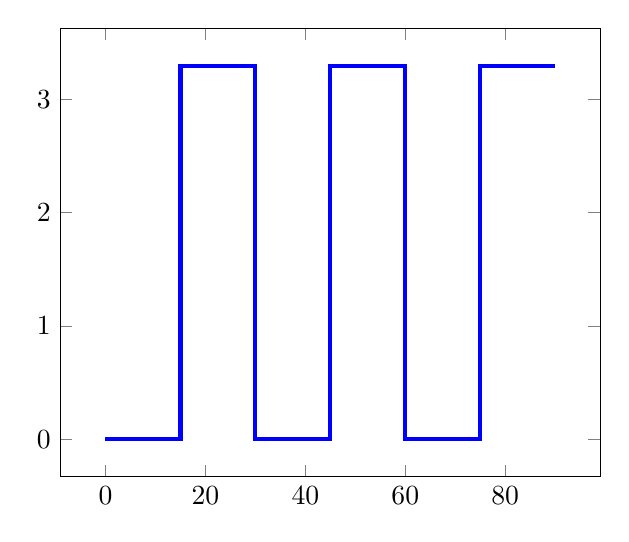
\begin{tikzpicture}
      \begin{axis}
        \addplot[color=blue, line width=1.5pt]  coordinates{(0, 0)(15, 0)(15, 3.3)(30, 3.3)(30, 0)(45, 0)(45, 3.3)(60, 3.3)(60, 0)(75, 0)(75, 3.3)(90, 3.3)};
      \end{axis}
    \end{tikzpicture}
    \label{Concept:Plot:square}
  } 

  % zigzag \foreach \x in {0, 15, ..., 90} {(\x, 3.3)}
  \subfloat[][Zick-Zack-Funktion]{
    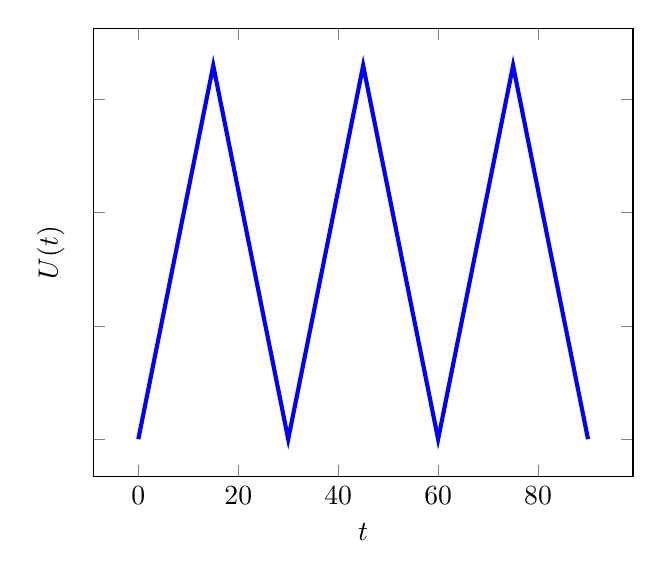
\begin{tikzpicture}
      \begin{axis}[yticklabels={$l$, , , , , ,$h$}, ylabel=$U(t)$, xlabel=$t$]
        \addplot[color=blue, line width=1.5pt] coordinates{(0, 0)(15, 3.3)(30, 0)(45, 3.3)(60, 0)(75, 3.3)(90, 0)};
      \end{axis}
    \end{tikzpicture}
    \label{Concept:Plot:zigzag}
  }
  % ramp
  \subfloat[][Rampenfunktion]{
    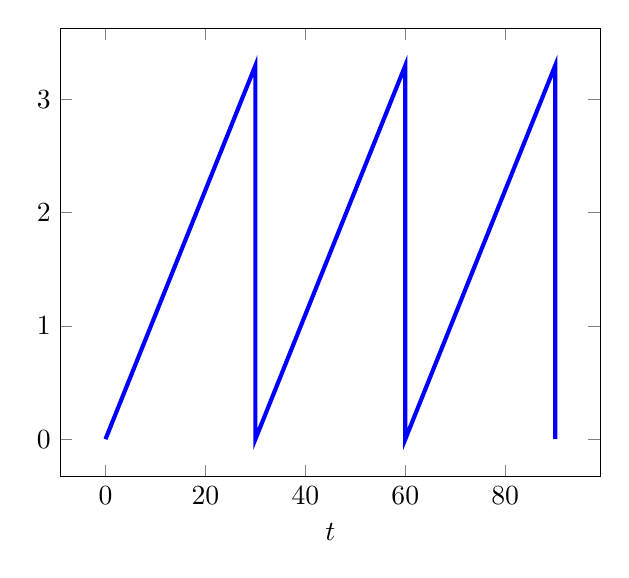
\begin{tikzpicture}
      \begin{axis}[xlabel=$t$]
        \addplot[color=blue, domain=0:90, line width=1.5pt]  coordinates{(0, 0)(30, 3.3)(30, 0)(60, 3.3)(60, 0)(90, 3.3)(90, 0)};
      \end{axis}
    \end{tikzpicture}
    \label{Concept:Plot:ramp}
  }
  \caption{Funktionen, die der Funktionsgenerator ausgeben kann. Ihr Verlauf ist als Spannung $U(t)$ über der Zeit $t$ aufgetragen. Die Zykluszeit und \analog{high} bzw. \analog{low} sind durch  $T$, $h$ und $l$ gekennzeichnet.} \label{Concept:Plot}
\end{figure}

\subsection{Konfiguration}
Der Funktionsgenerator muss, um extern konfiguriert werden zu können, über eine Möglichkeit zur Eingabe von Nutzerbefehlen verfügen.
Zu diesem Zweck wird die UART-Schnittstelle auf dem Basys 3-Board genutzt.
Über diese kann der Nutzer Konfigurationsbefehle per Computer versenden, die dann vom Generator interpretiert werden.

\section{Aufbau}

In \cref{Concept:FuncGenDia} wird der konzeptuelle Aufbau des Funktionsgenerators dargestellt.
Der Generator setzt sich aus verschiedenen Einzelkomponenten zusammen, die mit Signalen miteinander verknüpft werden.
Die Komponente, die für die Konfiguration zuständig ist (hier \code{CONFIG} gennant), ist über die Steuersignale \bitvect{cyc\_ticks}, \bitvect{high}, \bitvect{low}, \bitvect{thresh} und \bitvect{direction} mit den Funktionsbausteinen \code{CONST}, \code{SQUARE}, \code{ZIGZAG} und \code{RAMP} verbunden.
Darüber hinaus verfügt sie mit den Signalen \bit{RX} und \bit{TX} über Verbindungen zur UART Schnittstelle.
Das Signal \bitvect{waveform} steuert den Multiplexer, der das Ausgabesignal \bitvect{y\_out} an die interne Schnittstelle des DAC-Wandlers \code{DAC} weitergibt.
Diese Schnittstelle generiert daraus die Signale \lowactive{SYNC}, \bit{DINA}, \bit{DINB} und \bit{CLK} und transferiert sie dann an den DAC-Wandler.
Dieser wandelt sie anschließend in ein analoges Signal um.

\begin{figure}[h] \centering
  \includegraphics[width=1\textwidth]{function_generator} % , angle=-90, origin=c
  \caption{Diagramm des Funktionsgenerators. Aus Gründen der Übersichtlichkeit sind die \bit{CLK} Signale und \lowactive{CE} Signale nicht angeschlossen dargestellt. Alle \bit{CLK} Signale sind an den Systemtakt angeschlossen und alle \lowactive{CE} Signale liegen auf Masse.}  \label{Concept:FuncGenDia}
\end{figure}

